\chapter{Bogoliubov 模式与淬火协方差}
\label{ch:bogoliubov-quench}

\begin{learningobjectives}
完成本章后，读者应能：
\begin{enumerate}
  \item 把对称双分量凝聚体的线性涨落分解为密度与自旋通道；
  \item 由淬火前 Bogoliubov 真空构造淬火后的正常与反常协方差；
  \item 用旧基直接生成 Wigner 场样本，并检验新旧基之间的辛变换；
  \item 区分稳定准粒子压缩与动力学不稳定模的指数放大。
\end{enumerate}
\end{learningobjectives}

\section{均匀平衡背景}

本章采用标准弱涨落 Bogoliubov 线性化\cite{Dalfovo1999}。零模、有限体积
和数守恒问题需要更严格的投影处理\cite{Castin1998}；相干耦合双组分的物理
背景可参见\cite{Recati2022}。

先研究第14章均匀耦合模型，取失谐为零、无陷阱、总密度为 $n$，平均场背景为
\begin{equation}
  \psi_L^{(0)}=\psi_R^{(0)}=\sqrt{\frac n2}\,\ee^{-\ii\mu t/\hbar},
  \qquad
  \mu=\frac n2(g+g_{12})-J.
  \label{eq:balanced-two-component-background}
\end{equation}
定义对称与反对称涨落
\begin{equation}
  \delta\psi_d=\frac{\delta\psi_L+\delta\psi_R}{\sqrt2},
  \qquad
  \delta\psi_s=\frac{\delta\psi_L-\delta\psi_R}{\sqrt2}.
  \label{eq:density-spin-fluctuations}
\end{equation}
在 $g_{LL}=g_{RR}$、两分量平衡时，线性化哈密顿量在密度 $d$ 与自旋 $s$ 通道间分块对角。对自由色散
$\epsilon_k=\hbar^2k^2/(2m)$，下面把常被省略的中间步骤写出。先在旋转框架展开巨正则哈密顿量
$\hat K=\Hhat-\mu\hat N$，并令
\begin{equation}
  \delta\hat\Psi_c(x)=\frac1{\sqrt L}\sum_k\ha_{c,k}\ee^{\ii kx},
  \qquad c=d,s.
  \label{eq:density-spin-fourier-expansion}
\end{equation}
式\eqref{eq:balanced-two-component-background}使一阶项消失。把二阶项按无序波矢对 $\{k,-k\}$ 分组，可得
\begin{align}
  \hat K^{(2)}={}&\sum_{c=d,s}\sum_{k\in\mathcal K_+}
  A_{c,k}(\had_{c,k}\ha_{c,k}+\had_{c,-k}\ha_{c,-k})\notag\\
  &+\sum_{c=d,s}\sum_{k\in\mathcal K_+}
  B_{c,k}(\ha_{c,k}\ha_{c,-k}+\had_{c,k}\had_{c,-k})+\hat K_0,
  \label{eq:two-component-quadratic-pairs}\\
  A_{d,k}={}&\epsilon_k+\frac n2(g+g_{12}),
  &B_{d,k}={}&\frac n2(g+g_{12}),
  \label{eq:density-ab-coefficients}\\
  A_{s,k}={}&\epsilon_k+2J+\frac n2(g-g_{12}),
  &B_{s,k}={}&\frac n2(g-g_{12}).
  \label{eq:spin-ab-coefficients}
\end{align}
这里 $\mathcal K_+$ 从每一对非零波矢中只取一个代表；$\hat K_0$ 是必须单独处理的零模项。$2J$ 出现在自旋通道，是因为反对称单粒子态比凝聚的对称态高 $2J$；密度通道中的共同 $-J$ 已由化学势抵消。每个 $2\times2$ 动力学块满足
\begin{equation}
  \ii\hbar\partial_t
  \begin{pmatrix}\ha_{c,k}\\ \had_{c,-k}\end{pmatrix}
  =
  \begin{pmatrix}A_{c,k}&B_{c,k}\\-B_{c,k}&-A_{c,k}\end{pmatrix}
  \begin{pmatrix}\ha_{c,k}\\ \had_{c,-k}\end{pmatrix}.
  \label{eq:channel-bdg-dynamical-block}
\end{equation}
特征方程是 $E_{c,k}^2=A_{c,k}^2-B_{c,k}^2$，所以两支能谱为
\begin{align}
  E_d(k)^2&=\epsilon_k\left[\epsilon_k+n(g+g_{12})\right],
  \label{eq:density-bogoliubov-dispersion}\\
  E_s(k)^2&=(\epsilon_k+2J)
  \left[\epsilon_k+2J+n(g-g_{12})\right].
  \label{eq:spin-bogoliubov-dispersion}
\end{align}
密度支不依赖均匀 $J$，因为背景化学势与对称单粒子能量的 $J$ 位移抵消。自旋支在 $J>0$ 时有能隙；关闭 $J$ 后，若 $g_{12}<g$，它成为稳定的线性色散 Goldstone 模；若 $g_{12}>g$，一段低波数范围满足 $E_s^2<0$，背景发生动力学相分离不稳定。

\section{单个通道的 Bogoliubov 变换}

对每个通道与成对波矢 $\pm k$，二次哈密顿量可写成
\begin{equation}
  \Hhat_k^{(2)}=
  A_k(\had_k\ha_k+\had_{-k}\ha_{-k})
  +B_k(\ha_k\ha_{-k}+\had_k\had_{-k})+{\rm const.}
  \label{eq:paired-bogoliubov-hamiltonian}
\end{equation}
在 $A_k>|B_k|$ 时，$E_k=\sqrt{A_k^2-B_k^2}$ 为实数。取实系数约定
\begin{equation}
  \ha_k=u_k\hb_k-v_k\hbd_{-k},
  \qquad
  u_k^2-v_k^2=1,
  \label{eq:single-channel-bogoliubov-map}
\end{equation}
可选
\begin{equation}
  u_k=\sqrt{\frac12\left(\frac{A_k}{E_k}+1\right)},
  \qquad
  v_k={\rm sgn}(B_k)
  \sqrt{\frac12\left(\frac{A_k}{E_k}-1\right)}.
  \label{eq:bogoliubov-uv}
\end{equation}
若更换式\eqref{eq:single-channel-bogoliubov-map}中 $v$ 的符号约定，后续反常矩符号也会改变，但可观测协方差不变。代码中不应只保存 $E_k$；还要保存完整的模式相位与辛归一化约定。

式\eqref{eq:density-ab-coefficients}和\eqref{eq:spin-ab-coefficients}代入 $E_k^2=A_k^2-B_k^2$，分别复现式\eqref{eq:density-bogoliubov-dispersion}和\eqref{eq:spin-bogoliubov-dispersion}。这也说明两式不是独立记忆公式，而是同一个辛 $2\times2$ 块在两个通道中的结果。

\paragraph{$\pm k$ 的计数规则。}
式\eqref{eq:two-component-quadratic-pairs}若只对 $\mathcal K_+$ 求和，括号中必须同时保留 $k$ 与 $-k$；若改成对全部非零 $k$ 求和，整个成对哈密顿量要乘 $1/2$。抽样时 $b_k$ 与 $b_{-k}$ 是两个独立复高斯变量，不能因实值 Fourier 场的习惯而错误设置 $b_{-k}=b_k^*$：玻色场本身是复场。粒子--空穴伙伴只负责补全 Nambu 基，不再引入一套独立随机变量。$k=0$ 既等于自身的反向波矢，又可能是 Goldstone 模，必须从成对循环中剔除并按所选粒子数系综单独处理。

\section{突然淬火产生两模压缩}

设淬火前后参数分别记为 $i,f$。同一通道的两套系数是
$(u_{i,k},v_{i,k})$ 和 $(u_{f,k},v_{f,k})$。消去原子涨落算符后，新旧准粒子满足
\begin{equation}
  c_k=\mathcal A_k b_k+\mathcal B_k b_{-k}^\dagger,
  \label{eq:quench-mode-map}
\end{equation}
其中在上述实系数约定下
\begin{equation}
  \mathcal A_k=u_{f,k}u_{i,k}-v_{f,k}v_{i,k},
  \qquad
  \mathcal B_k=v_{f,k}u_{i,k}-u_{f,k}v_{i,k},
  \label{eq:quench-ab-coefficients}
\end{equation}
并满足 $\mathcal A_k^2-\mathcal B_k^2=1$。若初态是旧准粒子真空，则
\begin{equation}
  \qavg{\hat c_k^\dagger\hat c_k}=\mathcal B_k^2,
  \qquad
  \qavg{\hat c_k\hat c_{-k}}=\mathcal A_k\mathcal B_k,
  \label{eq:postquench-normal-anomalous}
\end{equation}
这里为简洁把新准粒子算符记作 $\hat c_k$。第一项是淬火产生的模式占据，第二项是相反动量之间的反常配对关联。对应量子态是相对于新真空的两模压缩高斯态。

有限温旧态的占据为 $\bar n_{i,k}$ 时，式\eqref{eq:postquench-normal-anomalous}推广为
\begin{align}
  \qavg{\hat c_k^\dagger\hat c_k}
  &=(\mathcal A_k^2+\mathcal B_k^2)\bar n_{i,k}+\mathcal B_k^2,\\
  \qavg{\hat c_k\hat c_{-k}}
  &=(2\bar n_{i,k}+1)\mathcal A_k\mathcal B_k.
  \label{eq:finite-temperature-quench-covariance}
\end{align}

\section{Wigner 协方差与直接抽样}

在 Wigner 表示中，旧准粒子样本为
\begin{equation}
  b_k=\sqrt{\frac{\bar n_{i,k}+1/2}{2}}
  (\xi_{1k}+\ii\xi_{2k}).
  \label{eq:old-mode-wigner-sample}
\end{equation}
把式\eqref{eq:quench-mode-map}中的算符替换为复数及其共轭，得到
\begin{equation}
  c_k=\mathcal A_k b_k+\mathcal B_k b_{-k}^*.
  \label{eq:new-mode-wigner-sample}
\end{equation}
其对称排序矩为
\begin{align}
  \ensavg{|c_k|^2}
  &=(\bar n_{i,k}+1/2)(\mathcal A_k^2+\mathcal B_k^2),\\
  \ensavg{c_kc_{-k}}
  &=(2\bar n_{i,k}+1)\mathcal A_k\mathcal B_k.
  \label{eq:new-mode-wigner-covariance}
\end{align}
第一式减去 $1/2$ 后正好得到式\eqref{eq:finite-temperature-quench-covariance}的正常占据。

实际 TWA 不必先生成新准粒子。更直接且较少出错的方法是用淬火前 BdG 模抽样，并立即重构原子场：
\begin{equation}
  \psi_\sigma(x,0)=\psi_\sigma^{(0)}(x)
  +\sum_{\nu\in\mathcal B_i}
  \left[u^{(i)}_{\sigma\nu}(x)b_\nu
  -v^{(i)*}_{\sigma\nu}(x)b_\nu^*\right].
  \label{eq:old-bdg-direct-field-sampling}
\end{equation}
随后直接用新哈密顿量的非线性场方程传播。新基协方差主要用于解析解释和抽样验收，而不是必需的中间数据格式。

\section{一般非均匀 BdG 问题}

在陷阱、SOC 或不对称耦合下，密度/自旋分块通常失效。设离散后有 $M$ 个空间--自旋单粒子模式。为与式\eqref{eq:old-bdg-direct-field-sampling}的负号约定一致，正能列及其粒子--空穴伙伴统一写成
\begin{equation}
  \bm w_\nu=\begin{pmatrix}\bm u_\nu\\-\bm v_\nu\end{pmatrix},
  \qquad
  \bar{\bm w}_\nu=\tau_x\bm w_\nu^*
  =\begin{pmatrix}-\bm v_\nu^*\\\bm u_\nu^*\end{pmatrix},
  \qquad
  \bm u_\nu=(u_{L\nu},u_{R\nu},\ldots)^T.
  \label{eq:general-bdg-mode-sign-convention}
\end{equation}
线性化方程具有广义辛本征结构
\begin{equation}
  \mathcal L\bm w_\nu=\epsilon_\nu\bm w_\nu,
  \qquad
  \bm w_\nu^\dagger\Sigma_z\bm w_\mu=\delta_{\nu\mu},
  \qquad
  \Sigma_z=\diag(\identity_M,-\identity_M).
  \label{eq:spinor-bdg-symplectic-norm}
\end{equation}
离散后要用与 TWA 相同的格点内积、规范和边界条件。普通 Euclidean 归一化 $\bm w^\dagger\bm w=1$ 不能保证准粒子对易关系。若 $\bm w_\nu$ 是能量 $+\epsilon_\nu$、辛范数 $+1$ 的模式，则式\eqref{eq:general-bdg-mode-sign-convention}中的 $\bar{\bm w}_\nu$ 具有能量 $-\epsilon_\nu$ 和辛范数 $-1$，其中 $\tau_x$ 交换 Nambu 的上下两块。

令 $U=(\bm u_1,\ldots,\bm u_M)$、$V=(\bm v_1,\ldots,\bm v_M)$。只有把 $M$ 个正范数模式及其 $M$ 个粒子--空穴伙伴同时放入，才得到可逆的完整伪幺正（paraunitary）矩阵
\begin{equation}
  \begin{aligned}
    \bm{\mathcal A}&=S\bm\beta,
    &\bm{\mathcal A}&=\begin{pmatrix}\bm a\\\bm a^\dagger\end{pmatrix},
    &\bm\beta&=\begin{pmatrix}\bm b\\\bm b^\dagger\end{pmatrix},\\
    S&=(\bm w_1,\ldots,\bm w_M,
    \bar{\bm w}_1,\ldots,\bar{\bm w}_M)
    =\begin{pmatrix}U&-V^*\\-V&U^*\end{pmatrix}.
  \end{aligned}
  \label{eq:complete-paraunitary-matrix}
\end{equation}
它必须满足
\begin{equation}
  S^\dagger\Sigma_zS=\Sigma_z,
  \qquad
  S^{-1}=\Sigma_zS^\dagger\Sigma_z,
  \qquad
  SS^{-1}=\identity_{2M}.
  \label{eq:paraunitary-identities}
\end{equation}
只把正能列排成一个 $2M\times M$ 矩阵时没有普通逆矩阵，不能直接写 $S^{-1}$。对淬火前后两个完整基，原子 Nambu 向量同时满足 $\bm{\mathcal A}=S_i\bm\beta_i=S_f\bm\beta_f$，所以
\begin{equation}
  \bm\beta_f=S_f^{-1}S_i\bm\beta_i.
  \label{eq:general-bdg-basis-map}
\end{equation}
用矩阵形式计算比逐个手写重叠公式更能容纳复模式、SOC 和简并子空间。简并正能子空间内还允许任意幺正旋转，因此跨参数匹配模式时应比较整个子空间投影，而不是依赖单列的相位或排序。严格零模、Jordan 块和复频不稳定模不能塞入上述普通 paraunitary 对角化；它们应先被投影出来，分别用数守恒集体坐标或线性辛时间传播处理。

\section{稳定压缩与不稳定放大}

“旧真空是新基中的压缩态”要求新二次哈密顿量存在实频率、正范数的稳定准粒子基。若式\eqref{eq:spin-bogoliubov-dispersion}给出 $E_s(k)^2<0$，相应模的频率为虚数，不存在以该不稳定背景为中心的正规新真空。此时仍可从旧态协方差出发，但应直接用线性辛传播
\begin{equation}
  V(t)=S_f(t)V(0)S_f(t)^T
  \label{eq:linear-covariance-propagation}
\end{equation}
或完整 TWA 演化。早期涨落指数增长是动力学不稳定，而不是平稳压缩准粒子振荡。非线性随后会饱和增长并耦合其他模式。

关闭 $J$ 还会使均匀自旋支的 $k=0$ 模成为零模。其 $u,v$ 在热力学参数化中可能发散，不能机械代入式\eqref{eq:bogoliubov-uv}。应改用相对相位--相对数的集体坐标，固定守恒粒子数扇区，或在有限体积数守恒 BdG 中单独处理。

\section{实际淬火协方差基准}

配套程序选取稳定参数 $g=1$、$g_{12}=0.6$，把均匀耦合从
$J_i=1$ 淬火到 $J_f=0.1$。程序直接抽样旧自旋准粒子真空，再变换到新基，比较正规占据和反常矩，结果见\cref{fig:bdg-quench-covariance}。
\begin{figure}[htbp]
  \centering
  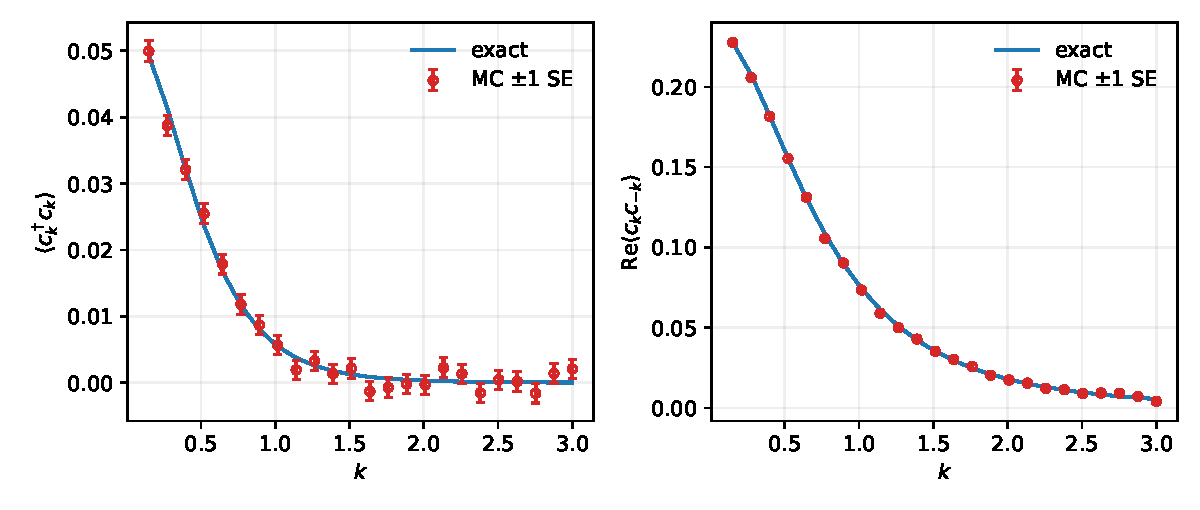
\includegraphics[width=0.78\textwidth]{figures/ch15/quench_covariance.pdf}
  \caption[BdG 淬火的正规与反常协方差基准]{在 $n=1$、$g=1$、$g_{12}=0.6$ 下，稳定自旋支从 $J_i=1$ 淬火到 $J_f=0.1$ 后的新基协方差。24个动量点各使用 $120000$ 对旧基真空样本，点的误差棒为 $\pm1$ 标准误，曲线为解析 Bogoliubov 变换；正规占据和反常矩的最大绝对误差分别为 $2.62\times10^{-3}$、$2.88\times10^{-3}$。同一运行还验收完整 paraunitary 矩阵、辛逆和原子场协方差；该图不覆盖零模或虚频不稳定区。}
  \label{fig:bdg-quench-covariance}
\end{figure}
图中点来自实际高斯 Monte Carlo；解析曲线由式\eqref{eq:quench-ab-coefficients}--\eqref{eq:new-mode-wigner-covariance}给出。全部参数与最大误差保存在
\path{data/ch15/quench_covariance_metrics.json}。同一程序还逐动量构造完整 $4\times4$
矩阵 $S_i,S_f$，验收 paraunitary 恒等式、辛逆矩阵、新旧基映射，以及由新旧基
重构原子 Nambu 协方差的一致性；因此图中的两条准粒子矩曲线不是唯一的通过条件。

\begin{chaptercheck}
完成 BdG 求解后先做四项机器测试：正负能成对、辛范数为正负一、不同正能模辛正交、由全部保留模重构投影单位算符。随后用至少一个稳定淬火比较“旧基直接抽样”和“新基协方差抽样”的原子场一、二阶矩。
\end{chaptercheck}

\section*{本章小结}

对称双分量凝聚体的线性涨落分成密度与自旋支，均匀耦合主要给自旋支开隙。稳定参数淬火把旧准粒子真空映射为新基中的两模压缩态，其正常与反常协方差由一个辛 Bogoliubov 变换确定。实际 TWA 可直接在旧基抽样并重构原子场。若新谱含虚频或零模，则应使用集体坐标或协方差传播，不能假定存在普通的新准粒子真空。

\begin{exercises}
  \item 从原始双分量哈密顿量逐项展开到式\eqref{eq:two-component-quadratic-pairs}，特别核对 $2J$、配对项以及只取 $\mathcal K_+$ 时的因子。
  \item 证明式\eqref{eq:quench-ab-coefficients}满足 $\mathcal A_k^2-\mathcal B_k^2=1$。
  \item 由式\eqref{eq:new-mode-wigner-sample}推导有限温协方差式\eqref{eq:new-mode-wigner-covariance}。
  \item 从式\eqref{eq:complete-paraunitary-matrix}证明式\eqref{eq:paraunitary-identities}，并说明为什么只保留正能列后不能求普通逆。
  \item 求 $J_f=0$、$g_{12}>g$ 时虚频波数区间。
  \item 设计一个数值测试，区分不稳定模的指数增长与稳定压缩模的周期振荡。
\end{exercises}
